
%(BEGIN_QUESTION)
% Copyright 2011, Tony R. Kuphaldt, released under the Creative Commons Attribution License (v 1.0)
% This means you may do almost anything with this work of mine, so long as you give me proper credit

Identify the types of instrument calibration errors shown in these graphs:

$$\includegraphics[width=15.5cm]{i01036x01.eps}$$

\vskip 20pt \vbox{\hrule \hbox{\strut \vrule{} {\bf Suggestions for Socratic discussion} \vrule} \hrule}

\begin{itemize}
\item{} Identify and sketch a calibration error other than the three represented here.
\item{} For each of the calibration errors shown, identify whether the error would be {\it positive} or {\it negative} in sign.
\item{} Explain how you may interpret any of these errors by inspection of tabulated numbers (i.e. without the benefit of a visual graph).  What numerical patterns, specifically, would you look for when identifying a zero error, or a span error, or any other type of calibration error?
\end{itemize}

\underbar{file i01036}
%(END_QUESTION)





%(BEGIN_ANSWER)

 
%(END_ANSWER)





%(BEGIN_NOTES)

From left to right: {\it zero shift}, {\it nonlinearity}, {\it span shift}

%INDEX% Calibration errors, identifying

%(END_NOTES)


